% Discussions & Conclusion
% Please delete the below lines and enter details for this assignment/homework
    Pour crée mes Feuilles de routes j’ai basé sur Package de l’arbre de
    Décision com.web.tree dans mon projet Accueil international .

\begin{enumerate}

\item Package: com.web.tree 
\begin{itemize}
\item Class Tree.java   : Contient les fonctions et les méthodes de creation et manipilation de notre arbre de décision .
Danns notre cas c'est une arbre de décision binaire avec quatre level inspire de l'exemple d'accueil international de Paris Saclay .


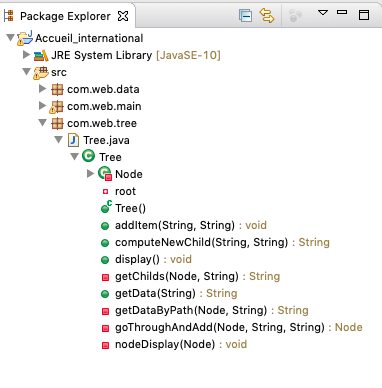
\includegraphics[scale=0.6]{Images/ad.png}

   
\end{itemize}


\item Package: com.web.data

\begin{itemize}
\item Class Chapitre.java : Stucture de base de notre fuille de route
\\Titre : Titre de Chaque Chapitre exemple Logement, Inscription .
\\ Contenu : Déscription de Chapitre .
\\DElais : délais a respecter pour le démarche adminstrative .

\item Class FeuilleDeRoute.java  :  Creation et affichage de feuille de route
selon l'index (index c'est le nombre des chapitres dans une feuille de route selon chaque cas ) .
\\

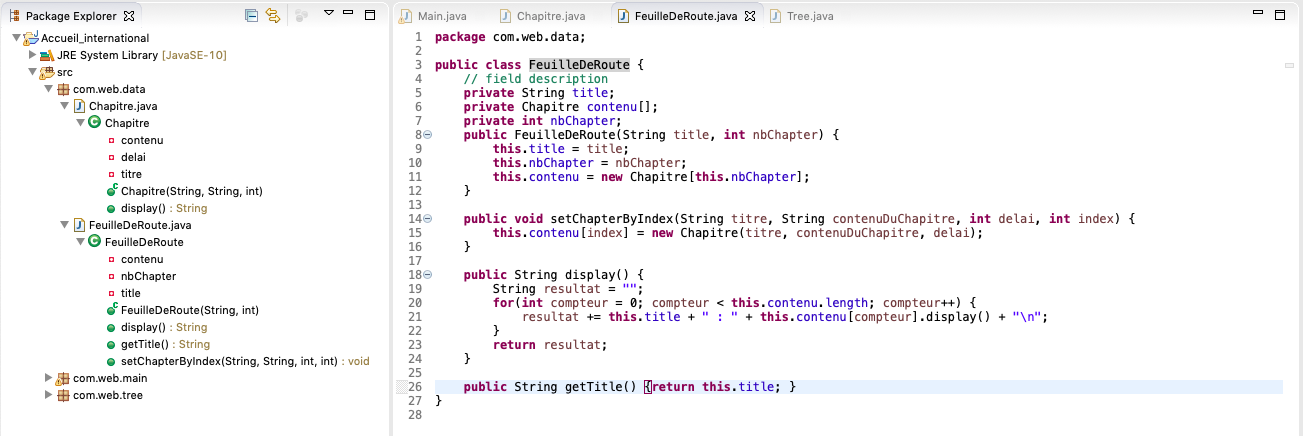
\includegraphics[scale=0.3]{Images/fdr.png}



   
\end{itemize}

\item Package: com.web.main  : Programme Principale 


 public static void main(String agrs[])
\\ Tous les fonctions de cration et affichage d'arbre de décisions et feuille de route .
\\Creation des feuille de route selon les feuille de notre arbre de décision.


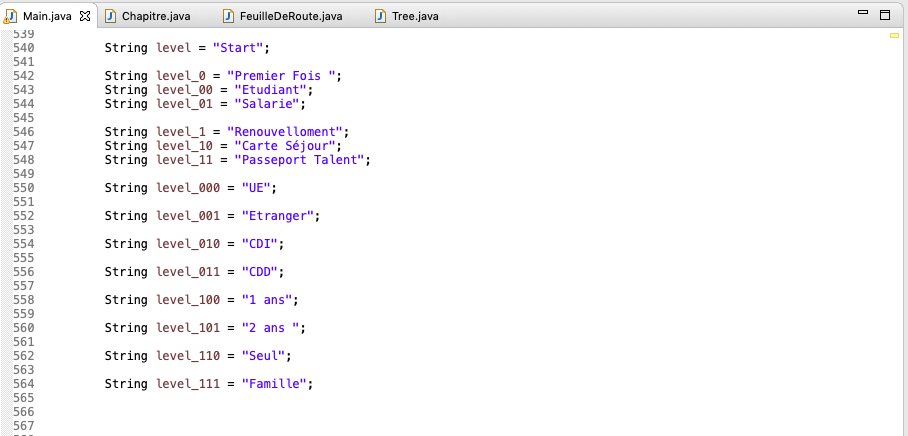
\includegraphics[scale=0.3]{Images/main.png}



   



\end{enumerate}
